\documentclass{beamer}
\mode<presentation>
\usepackage{amsmath}
\usepackage{amssymb}
%\usepackage{advdate}
\usepackage{graphicx}
\graphicspath{{../figs/}}
\usepackage{adjustbox}
\usepackage{subcaption}
\usepackage{enumitem}
\usepackage{multicol}
\usepackage{mathtools}
\usepackage{listings}
\usepackage{url}
\def\UrlBreaks{\do\/\do-}
\usetheme{Boadilla}
\usecolortheme{lily}
\setbeamertemplate{footline}
{
  \leavevmode%
  \hbox{%
  \begin{beamercolorbox}[wd=\paperwidth,ht=2.25ex,dp=1ex,right]{author in head/foot}%
    \insertframenumber{} / \inserttotalframenumber\hspace*{2ex} 
  \end{beamercolorbox}}%
  \vskip0pt%
}
\setbeamertemplate{navigation symbols}{}
\let\solution\relax
\usepackage{gvv}
\lstset{
%language=C,
frame=single, 
breaklines=true,
columns=fullflexible
}

\numberwithin{equation}{section}
\title{4.12.6}
\author{AI25BTECH11001 - ABHISEK MOHAPATRA}
% \maketitle
% \newpage
% \bigskip
\begin{document}
{\let\newpage\relax\maketitle}
\renewcommand{\thefigure}{\theenumi}
\renewcommand{\thetable}{\theenumi}


	 	\textbf{Question}:
The owner of a milk store finds that he can sell 980 litres of milk each week
at 14/litre and 1220 litres of milk each week at 16/litre. Assuming a linear
relationship between selling price and demand, how many litres could he sell weekly
at 17/ litre?

		\textbf{Solution:} 
Let the litres at 17/ litre be x.
Representing the data, Let
\begin{align}
\vec{A} = \myvec{980 \\ 14},
\vec{B} = \myvec{1220 \\ 16},
\vec{C} = \myvec{x \\ 17}
\end{align}

so as per the question these point lies on a line,
\begin{align}
	\Rightarrow rank\myvec{\vec{A}-\vec{B} & \vec{C}-\vec{B}}^\top = 1 
\end{align}

\begin{align}
	\Rightarrow \myvec{\vec{A}-\vec{B} & \vec{C}-\vec{B}}^\top = \myvec{-240 & -2 \\ x-1220 & 1} 
\end{align}
\begin{align}
	\xleftrightarrow[]{C_1\xleftrightarrow[]{} C_2} \myvec{-2 & -240 \\ 1 & x - 1220}
\end{align}
\begin{align}
	\xleftrightarrow[]{R_2\rightarrow R_2 + \frac{1}{2}R_1} \myvec{-2 & -240 \\ 0 & x - 1340}
\end{align}

so for rank = 1, x = 1340.

1340 litres is the required answer.


Graph:
\begin{figure}[h!]
	\centering
	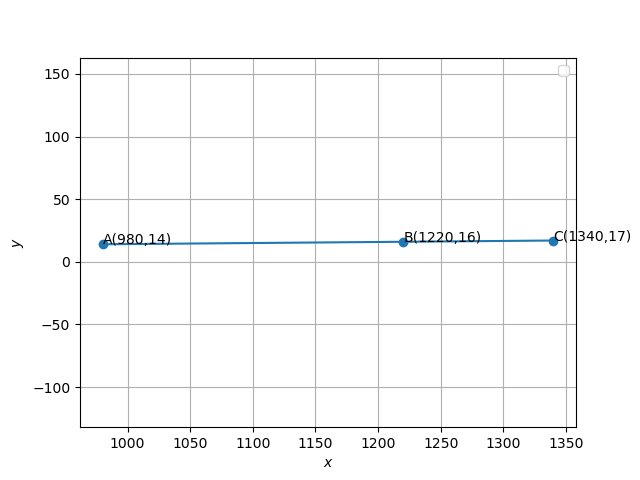
\includegraphics[width=0.7\linewidth]{fig1.png}
\end{figure}
\end{document}
